\documentclass[../../../../main.tex]{subfiles}
\begin{document}

一辺の長さが $\ell$ の正方形の内部に半径1の円が入っている．
ここで $\ell>2$ とする．
この円が図のように正方形の角から出発して正方形の辺にそってすべらずに正方形の内部をころがる．
ただし円が正方形の他の辺に接すれば次にはその辺にそってすべらずにころがるとする．
この円の中心が最初にもとの位置にもどってくるまでの円周上の点 $P$ の軌跡を考える．

\begin{figure}[htbp]
  \centering
  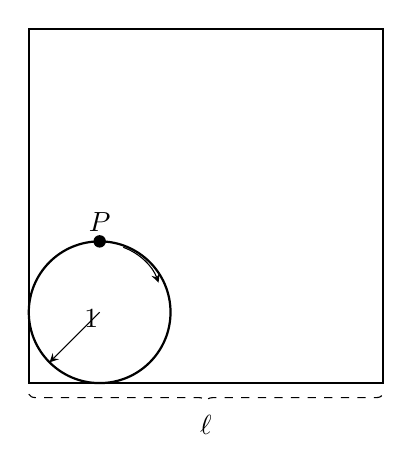
\begin{tikzpicture}[scale=1.5, >=stealth]
    \draw[thick] (0,0) rectangle (3,3);

    \coordinate (O) at (0.6, 0.6);
    \draw[thick] (O) circle (0.6);

    \draw[->] (O) -- (0.176, 0.176) node[midway, above right] {$1$};

    \coordinate (P) at (0.6, 1.2);
    \fill (P) circle (1.5pt) node[above] {$P$};

    \draw[->] (0.8, 1.15) arc (70:20:0.5);

    \draw[dashed, decorate, decoration={brace, mirror, raise=4pt}] (0,0) -- (3,0) node[midway, below=8pt] {$\ell$};
  \end{tikzpicture}
\end{figure}

\begin{enumerate}
  \item $P$ の軌跡の始点と終点が一致するための $\ell$ の条件を求めよ．
  \item $\ell$ は (1) の条件を満たす最小の長さとする．
  このとき $P$ の軌跡の長さのとりうる値の範囲を求めよ．
\end{enumerate}

\end{document}
